\chapter{Problem Analysis}
\label{problemanalysis}

For the scope of our project, we define all citations as belonging to one of two types: \textbf{General} and \textbf{Specific}. 
% Min: didn't quite get this sentence.  What does it mean?
We define citations as such to be inline with our goal. That is, given a citation as Specific, that there is a specific portion of the cited document that contains the original information to support the citation. Otherwise, the citation is General. We use the following guideline to ensure that there is no ambiguity in our definition of the dichotomy between General and Specific: \\ \\
\textbf{General Citations}
\begin{enumerate}
\item Authors may refer to a paper as a whole. If the author cites the cited paper for a key idea, e.g. Machine Learning, and Machine Learning makes up the entire or majority of the cited paper, it is a general citation.
% Min: do you want to be more specific about "contributions"?
\item Authors may refer to a paper as a form of mentioning. In such cases, the authors merely mention the cited paper to acknowledge its contributions.
\end{enumerate}
\textbf{Specific Citations}
\begin{enumerate}
\item Authors may refer to a term definition in the cited paper.
\item Authors may refer to a key idea/implementation in the cited paper. This key idea or implementation does not constitute the entire or majority of the cited paper.
\item Authors may refer to an algorithm or a theorem in the cited paper. This algorithm/theorem and its supplementary evidence does not constitute the entire or majority of the cited paper.
\item Authors may refer to particular digits or numerical figures in the cited paper. This is usually done to make reference to quantitative evaluation results in the cited paper. Authors may also complement the cited paper for its performance.
\item Authors may quote a passage in the cited paper.
\end{enumerate}

\begin{figure}[h]
\label{fig:terminology}
\framebox[\textwidth]{
	\begin{tabular}{ l p{11cm}}
		\textsc{Term} & \textsc{Description}\\
		\hline
% Min: need to define "in-line citation"?
		Citing Paper & The paper that makes the citation \\
		Cited Paper & The paper that is being cited by the citing paper \\
% Min: you need to make sure that the format Xdd-dddd is known to the reader as standing for a paper.
% Min: if possible, show these relationships also in a graphical figure.  You can use powerpoint or something to draw and export as a .eps or .pdf
		Cite Link & E.g. \url{E06-1034==>J93-2004}. A citation relation between a citing paper (\url{E06-1034}) and a cited paper (\url{J93-2004}) \\
		Cite String & The citation mark. E.g. Nivre and Scholz (2004), [1], (23) \\
		Citing Sentence & A sentence in the citing paper that contains the in-line citation. E.g. \textit{That algorithm, in turn, is similar to the dependency parsing algorithm of \textbf{Nivre and Scholz (2004)}, but it builds a constituent tree and a dependency tree simultaneously.} \\
		Citing Context & The block of text surrounding the citing sentence, about 2 sentences before and after the citing sentence, for providing contextual information \\
		Cited Fragment & A fragment, from a few lines to paragraphs, in the cited paper
	\end{tabular}
}
\caption{Terminological conventions used in this dissertation}
\end{figure}

% Min: not clear.  Is this the goal, what is already done or what is to be done?
For \textbf{Specific} citations, we specifically extract a fragment in the cited paper that represents the source of the information mentioned in the citation itself, i.e. citation provenance.

\section{Scope Of The Problem}
We decompose the task into two tiers.  In the first tier, we first determine whether a citation is General or Specific. If a citation is General, the reader can be directed, for example, to the abstract of the cited paper. If a citation is Specific, the reader can be directed to the specific paragraph or line.  From our definition, given that a citation is Specific, then there must exists a region in the cited paper that the citation refers to. To solve this second tier, we implement a ranking system that determines the location of this region.

Our project has a practical aspect that can be readily applied to scholarly papers.  However, even with the components above, to field the project practically, the system must be able to detect in-line citations in a suitable textual representation of a scholarly paper corpus. 
While such engineering issues are important, our work focuses only on the research aspects of determining citation provenance, and hence we abstracted away the problem of locating in-line citations.  Instead we reduced the problem to only determining the type of a citation and its location. To solve the practical problem of locating the in-line citations, we utilize the open-source logical document structure and reference string parsing system, ParsCit, developed in \outcite{parscit}. Conveniently, ParsCit identifies the citing sentence, together with its citing context.

\section{Modelling The Problem As Search}
In web search engines, an user enters a search query, and a search engine would use this query to search within its search domain -- millions of web pages -- and then display the best matching web pages as compared to the search query. 
% Min: unclear.  What do you mean "having a search query"?
That would be equivalent to having a search query for an entire corpus of research papers. Our second subproblem of linking Specific citations to their origin can be modelled as search.

Consider reading a paper, \url{A}. We know the citations made by \url{A}, and these cited papers are listed in its References section. From this our search domain for any query from \url{A} would be the contents of the list of cited papers. We reduce this search domain further when we are investigating a particular citation in \url{A}, say now paper \url{A} cites the paper \url{B}. Now, for this citation, the scope of search would be the sub-domain -- contents of paper \url{B}. So instead of searching for the best matching document in the corpus, we are now searching within \url{B}. The search query is the citation from \url{A}, and the {\it candidate documents} are the various regions (fragments) in \url{B} (Refer to Figure \ref{fig:model} for a simple illustration). With the help of ParsCit \cite{parscit}, the citing context can be extracted. The search query is then citing context which consists of the citing sentence.

\begin{figure}[h]
  \centering
  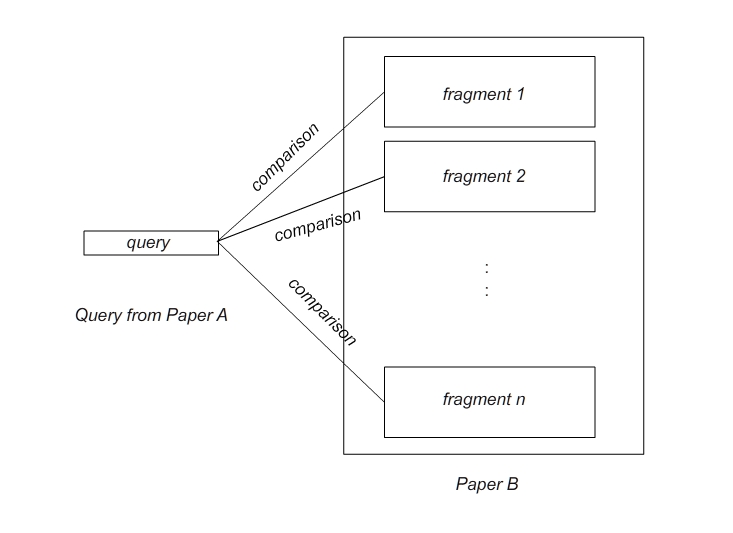
\includegraphics[scale=0.50]{./model}
  \caption{Modeling Our Problem}
  \label{fig:model}
\end{figure}

Cast this way, our first subproblem is simply a \textit{binary classification problem}, where we attempt to determine whether a fragment is either General or Specific.

\section{Target Corpus}
\label{buildingcorpus}
We selected the ACL Anthology Reference Corpus\footnote{http://acl-arc.comp.nus.edu.sg/} (ACL-ARC) as the target corpus to perform our research on. The ACL-ARC consists of publications covering topics in computational linguistics.  While we wish to generalize our citation provenance methodology to work on publications from all fields of research, we chose to start with this corpus as it provides the \textit{interlink data} that conveniently informs us of the cite links between the papers in the corpus. For instance, in the interlink data, a link like \url{X98-103==>X96-1049} says that the paper \url{X98-103}\footnote{All ACL-ARC papers are assigned an unique paper ID} cites \url{X96-1049}.  

% Min: the $n$ factor is usually very small so it doesn't seem O(nm).  Rather instead of the $n$ citing contexts it is that there are $k$ references.  The complexity is then mostly dominated by O(km)
Given our formal problem statement, we can now specify the required data for the task. For each cite link, there can be multiple in-line citations i.e. multiple citing contexts, when a target paper is cited multiple times by the authors. Each citing context is compared with every fragment in the cited paper; i.e., if a cite link has $n$ citing contexts and the cited paper can be divided into $m$ fragments.  This immediately gives rise to $(n \times m)$ data instances.
% Min: show some examples of data instances.

% Min: you need to give some reasoning about why annotations are needed before proceeding into the annotations themselves.
% Min: GLOBAL you still tend to use passive tense and modals.  Try to use active and simple tenses.
% Min: GLOBAL use \url.  I've fixed one URL below.  Don't use URL for non-URLs because in PDFs the URLs will be active hyperlinks (that then won't work)
\subsection*{Collecting Annotations -- First Attempt}
The first attempt at collecting annotations was to require an annotator to specify the line numbers of the cited information that the citing context was referring to. The annotator would be provided the citing and cited paper in plain text format, and he/she will need to annotate on a separate file, specifying the line number range, e.g. line range \url{L12-55} of the cited paper. For this annotation task, we designed an annotation framework\footnote{\url{http://citprov.heroku.com}} where an annotator is presented with an user-friendly interface to select the lines in the cited paper that he/she deem Specific. We posted this task onto the Amazon Mechanical Turk (MTurk\footnote{https://www.mturk.com}) as an attempt to collect annotations on a larger scale and we collected some annotations from a few MTurk workers. After a trial round of annotation, we reviewed this annotation scheme together with feedback from the small group of participants.

% Min: I recall you did an IRB application.  You should mention that, especially if it was approved to be exempted.  That is a significant amount of effort.
First, this annotation task is non-trivial. Participants must be able to understand the contents of the papers, and thus, must largely be either subject matter experts (researchers) or have some experience in reading scientific papers. While it is possible to target a selected category of MTurk workers for this task, the complexity of this task requires participants with research experiences, which could be limited in numbers. Furthermore, most of the annotations collected from MTurk do not agree among the annotators and ourselves. Thus we abandoned collecting annotations via MTurk, and performed annotations manually.

Second, this annotation scheme is too tricky, and would also cause us much problem when it comes to evaluation. Consider an implemented system that outputs a prediction for citation provenance in the form of a line number range. It is difficult to judge the correctness of this prediction, say \url{L50-78}, when compared against the annotated \url{L12-55}. The prediction \textit{overlaps} the annotation by 5 lines, but this variable amount of overlap is not definitive and difficult to decide at what extent of overlap only do we consider the prediction correct. Thus we switched to the alternative.

\subsection*{Collection Annotations -- Second Attempt}
The second attempt is more straightforward. Recall that we used ParsCit for extracting the citing context. ParsCit also divides a paper into logically adequate fragments according to sections, sub-sections, figures and tables etc. So instead of annotating the papers in plain text format by line number ranges, we annotated the structured output from ParsCit, each of the fragments of the cited papers with 3 classes: General ($g$), Specific-Yes ($y$) and Specific-No ($n$). To be precise, we annotated $g$ (for all its fragments) if a cite link is deemed General, and $y$ \underline{only} for the fragment(s) that is deemed Specific. For the other fragments that are not Specific, we annotated $n$. Table \ref{tab:annotation} summarises the statistics for annotation. Note that only percentage values for Specific instances are displayed.

\begin{table}[h]
	\center
	\begin{tabular}{ l | l}
		\textsc{Item} & \textsc{Statistics}\\
		\hline
		No. of Cite Links & 275 (7.6\% Specific) \\
		No. of Fragments & 30943 (0.09\% Specific-Yes, 12.9\% Specific-No)
	\end{tabular}
	\caption{Annotation Statistics}
	\label{tab:annotation}
\end{table}

Specific citations are very rare and the training data is heavily skewed towards General citations. After prolonged periods of searching for valid Specific citations in our training corpus, we argue that despite more attempts to gather more positive instances, the ratio between General and Specific would remain the same. This challenging situation we have with the annotations also contributes to our approach to the problem, as we explain in the following chapter.

During the annotation process, we observed that Specific citations can be categorised into four sub-classes.  We acknowledge that these observations are limited to the particular corpus we worked with and may not generalize.  We observed that Specific citations may:
\begin{enumerate}
\item refer to digits/numerical figures in the cited paper, usually in the evaluation section
\item refer to term definitions by the author(s) of the cited paper
\item refer to algorithms/theorems in the cited paper
\item quote a line or segment in the cited paper
\end{enumerate}
These observations also led to the implementation of some features that are defined next chapter in our approach.
